\problemname{Knockout Tournament}

Laura is organising a knockout tournament, in which her friend Dale takes part.
Laura would like to maximise the probability of Dale winning the tournament by
arranging the games in a favourable way. She does not know how to do it, so she
asked you for help. Naturally, you refuse to cooperate with such a deplorable
act---but then you realise that it is a very nice puzzle!

When the number of players is a power of two, the tournament setup can be
described recursively as follows: the players are divided into two equal groups
that each play their own knockout tournament, after which the winners of both
tournaments play each other. Once a player loses, they are out of the
tournament.

When the number of players is not a power of two, some of the last players in
the starting line-up advance from the first round automatically so that in the
second round the number of players left is a power of two, as shown in
Figure~\ref{fig:knockout}.

\begin{figure}[h!]
  \centering
  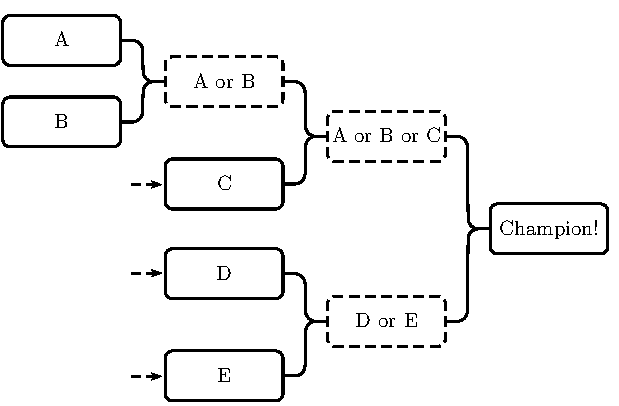
\includegraphics[width=0.5\textwidth]{sample2}
  \caption{A tournament tree with $5$ players.  Players C, D, and E advance from the first round automatically.}
  \label{fig:knockout}
\end{figure}

Every player has a rating indicating their strength.
A player with rating $a$ wins a game against a player with rating $b$ with
probability $\frac{a}{a+b}$ (independently of any previous matches played).

Laura as the organiser can order the starting line-up of players in any way she
likes. What is the maximum probability of Dale winning the tournament?


\section*{Input}

The input consists of:
\begin{itemize}
  \item One line with an integer $n$ ($2 \le n \le 4096$), the total
    number of players.
  \item $n$ lines, each with an integer $r$ ($1 \le r \le 10^5$), the
    rating of a player. The first rating given is Dale's rating.
\end{itemize}


\section*{Output}

Output the maximum probability with which Dale can win the
tournament given a favourable setup. Your answer should have an absolute or
relative error of at most $10^{-6}$.
